\section{Internet of things}
Cluster of European research projects regarding the Internet of Things:
\begin{quote}
    'Things' are active participants in buissness, information and social processes where they are enabled to interact and communicate aming themselves and with the enviorment by exhchanging data and information sensed about the envoirment while reacting autonomously to real/physical world events and influencing it by runnign processes that trigger actions and create services with or without direct human intervention.\cite{Gubbi2013}
%Fix correct qoute on this!
\end{quote} 

Gubbi et. al. defines the Internet of Things as:
\begin{quote}
    Interconnection of sensing and actuating devices providing the ability to share inforamtion across platforms through a unified framework, developing a common operating picture for enabling innovative applications. 
    This is achieved by seamless large scale sensing, data analytics and information representation using cutting egde ubiquitous sensing and cloud computing.\cite{Gubbi2013}
\end{quote}

\section{Industry 4.0}
%Industry 4.0 definition.
Lasi argues that the term industry 4.0 was coined beforehand as a planned fourth industrial revolution.\cite{Lasi2014}
The use of internet of things devices, IoT devices from now on, and cyber-physical systems, CPS from now on is what defines the fourth industrial revolution Vadiya means.\cite{Vaidya2018}
See figure x for a short historic overview of previous industrial revolutions.   
\begin{figure}
    \centering
    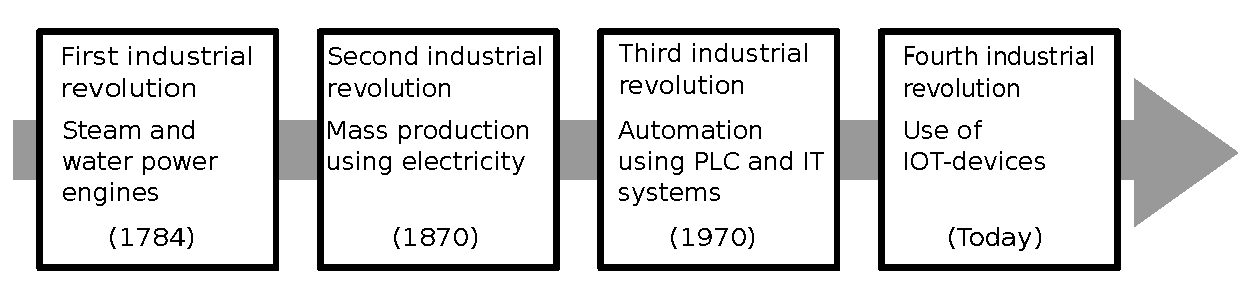
\includegraphics[width=\textwidth]{Pictures/Industrial_revolution.pdf} 
    \caption{Historic overview of previous industrial revolutions}
    \label{Indutrial revolutions}
\end{figure}

According to Vadiya industry 4.0 promotes the connection of sensors and devices both to the internet and to other sensors or devices.\cite{Vaidya2018} 

%Intelligent  sensors.
Hozdić states that a sensor is a device capable of providing an appropriate output in response to a measured value.
One key feature of an intelligent sensor is that to increase the level of information processing it processes the information at a logical level Hozdić argues.
An Intelligent sensor  is capable of executing actions based on the measured value in contrast to regular sensors, making them easier to set up and use means Hozdić.\cite{Hozdic2015} 

%Cyber Physical Systems (CPS).
Hozdić defines a cyber-physical system, CPS, as a new generation of a system that integrates both physical and computer abilities.
A cyber-physical system consists of two parts, one cybernetic and one physical.
The cybernetic part of the system can be viewed as a summation of logic and sensor units while the physical part of the system can be viewed as a summation of the actuator units Hozdić adds.
Xu et. al. states that cyber-physical systems are a key part of Industry 4.0. In contrast to the simple embedded systems of today will be exceeded due to advances in CPS that enable enhanced capability, scalability, adaptability, resiliency, safety, usability, and security.\cite{Xu2018}
Hozdić argues that the CPS can share and receive information from intelligent sensors that connect to digital networks is what enables and form an internet of things.\cite{Hozdic2015}
 
\section{Arrowhead framework}
%Local cloud.
A local cloud is defined as a self-contained network with at least the three mandatory systems deployed, more on those in a later paragraph. 
Delsing et.al. also argues that the three mandatory core systems running a local cloud also need at least one application system deployed.\cite{Delsing2017}

%Service and systems.
Two terms have to be introduced to further understand what the Eclipse Arrowhead framework aims to accomplish, services and systems.
Delsing et. al. defines a system as what is providing or consuming a service.
Furthermore, a service is defined as what is used to convey information between a provider and a consumer Delsing et. al. argues.\cite{Delsing2017}

%Mandatory core systems.
The Eclipse Arrowhead framework, Arrowhead from now on, consists of three mandatory core systems according to Delsing et. al.
To fully operate a local cloud as defined in the previous section it must, according to Delsing, contain:
\begin{itemize}
    \item Service registry system.
    \item Authorization system. 
    \item Orchestration system.\cite{Delsing2017}
\end{itemize} 

\begin{figure}[H]
    \centering
    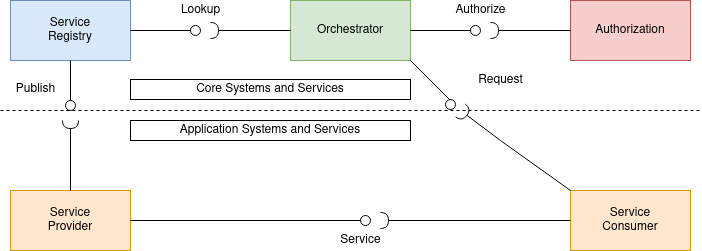
\includegraphics[width=\textwidth]{Pictures/arrowheadfulldiagram.png} 
    \caption{The core systems of the Eclipse Arrowhead framework}
    \label{diagram arrowhead}
\end{figure}
More about the dynamics betweeen the consumer and provider system will follow in the theory section.
\section{Amazon Web Services}

\begin{figure}[H]
    \centering
    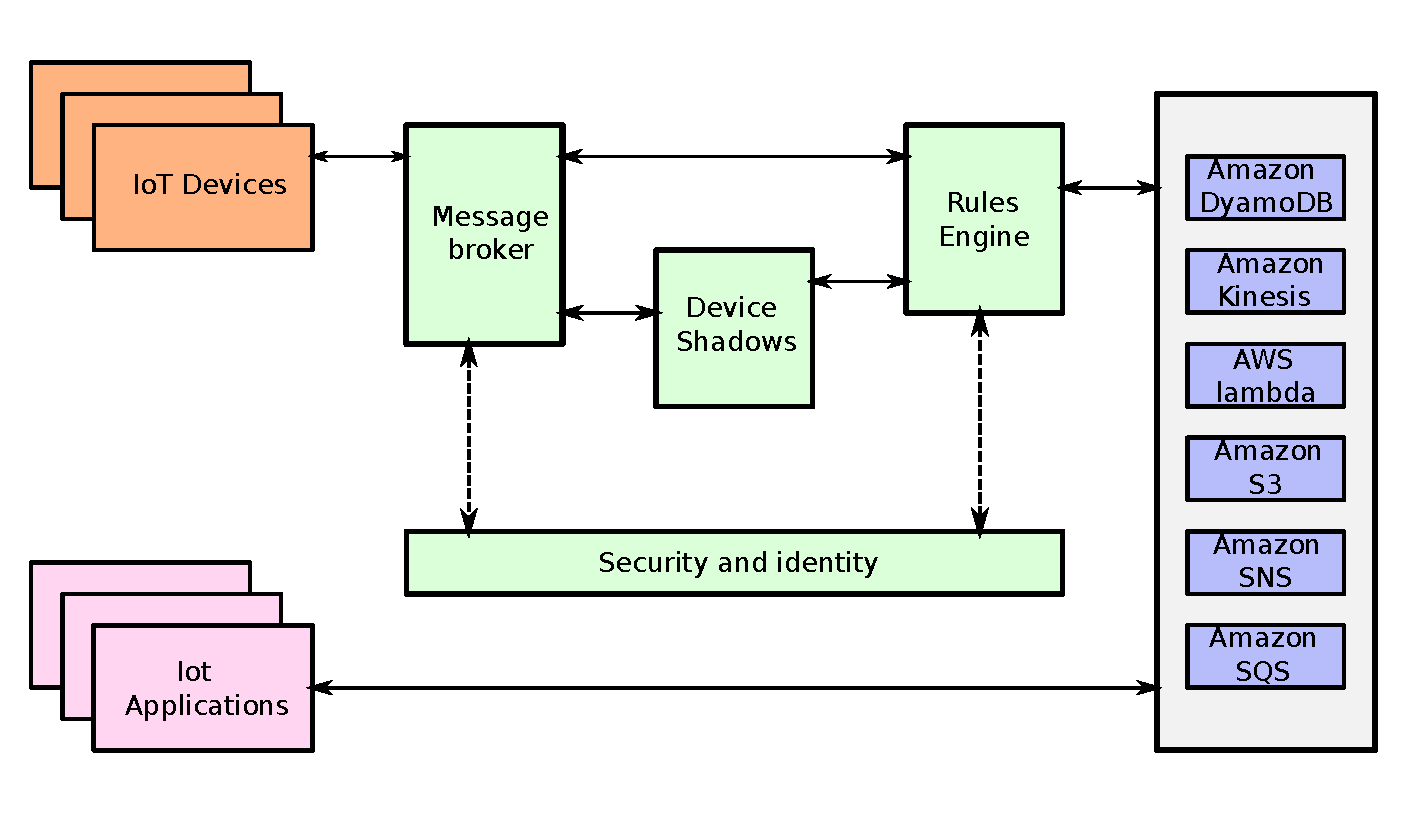
\includegraphics[width=\textwidth]{Pictures/aws.pdf} 
    \caption{The core systems of the Amazon Web Services}
    \label{diagram AWS}
\end{figure}
\section{Security}
%Introduction.
Meneghello et. al. argues that the increasing number of IoT devices and the pervasive nature of new smart home or healthcare devices can pose a real threat to the users' integrity.
Sensitive information Meneghello et. al. defines as a video recording of the user's home, the user's location, access to buildings, health monitoring, and industrial processes.\cite{Meneghello2019}

%Secruity challenges.
Meneghello et. al. states the security requirements of an IoT system can be divided into three different operational levels, namely the information, access, and functional level.
The information level should guarantee that the integrity, anonymity, confidentiality, and privacy of the system are preserved. 
Meaning that messages should not be altered during transmission, the identity of the data source and the clients' private information remains hidden and that data cannot be read by third parties Meneghello et. al. argues.
The access level provides a guarantee that only legitimate users are allowed access to the network and the devices associated with that network. 
It also guarantees that users within the network only use resources they are allowed to use Meneghello et. al. states.
The functional level should guarantee the continued functionality of a network even in the case of malfunction or a malicious attack Meneghello et. al. adds.\cite{Meneghello2019}

%Pricacy.
Zhang also argues that privacy is a big concern with IoT devices and suggests two solutions data collection policy and data anonymization.
A policy that describes how the data is collected from the devices would restrict the flow of data, therefore ensuring privacy preservation can be ensured Zhang states.
Data anonymization means that the private information sent by the IoT devices is either encrypted or that the relation of the data and its owner is concealed according to Zhang.\cite{Zhang2014}

%Encryption.
Meneghello et. al. argues that one of the main aspects of security within IoT is to ensure that the data sent is the data received and that the data has not been tampered with or read during transmission.
The most important operation to guarantee that is the use of encryption, which converts the message sent in plain text to an encrypted message only readable with a decryption key Meneghello et. al. states.
Meneghello et. al. states that there are two mechanisms for encryption, symmetric and asymetric.
Symmetric encryption is when the same key is used for encryption and decryption, so it has to be shared with both the sender and receiver.
Asymmetric encryption on the other hand only shares the public key and the sender and receiver have their own private keys Meneghello et. al. means.\cite{Meneghello2019}

%End-to-End encryption.
Hassija et. al. states the importance of end-to-end encryption and the challenges it poses for IoT systems.
End-to-end encryption is required to ensure the confidentiality of the data, the application should not let anyone except the intended recipient read the messages sent Hassija adds.\cite{Hassija2019}

%Authentification.
Noor, Meneghello, and Zhang state the importance of authentification in IoT systems.\cite{Noor2019,Meneghello2019,Zhang2014} 
Noor adds that 60\% of all IoT systems use authentification to grant access to the user.\cite{Noor2019}  
Zhang argues that public key cryptosystem provides more security compared to symmetric encryption schemes, but has the drawback of having high computational overhead.\cite{Zhang2014} 

%Lightweight cryptography.
Noor argues that conventional cryptographic primitive is unsuitable for IoT devices due to their lack of computational power and limited battery life and memory capacity.\cite{Noor2019}
With IoT devices lacking capabilities as background Noor, Meneghello, and Zhang all agree that a push for lightweight cryptography is required to ensure the security of these devices.\cite {Noor2019,Meneghello2019,Zhang2014} 

\section{Communication} 
%MQTT
MQTT, Message Queue Telemetry Transport, is a lightweight messaging invented by IBM suitable for IoT Wukkadada means.\cite{Wukkadada2018} 
MQTT is a publish/subscribe protocol that requires a minimal footprint and bandwidth to connect an IoT device according to HIVEMQ.\cite{MQTT2021}
MQTT consists of an MQTT broker and MQTT clients, where the broker is responsible for sending messages between the sender and its recipients.\cite{Wukkadada2018}
A client on the other hand publishes a message to the broker that other clients can subscribe to HIVEMQ adds.\cite{MQTT2021}

%HTTP/HTTPS
HTTP, HyperText Transfer Protocol, is a request/response protocol consisting of clients and servers that communicate by exchanging individual messages. 
The clients are responsible for the requests and the servers are responsible for the response Mozilla developer network clarifies. \cite{HTTP2021} 
In contrast to the lightweight MQTT protocol with low overhead and bandwidth, HTTP can cause serious bandwidth issues Wukkadada adds. \cite{Wukkadada2018}
The biggest benefits to using HTTP are that it supports the RESTful Web architecture and that it is a globally accepted web messaging standard Naik suggests. \cite{Naik2017} 

%Comparisson 
Naik argues that HTTP exceeds MQTT in message size, message overload, power consumption, resource requirements, bandwidth, and latency. 
All things that are considered negative for a protocol.
On the other hand, HTTP exceeds MQTT in interoperability, standardization, security, and provisioning Naik adds.\cite{Naik2017}
All things that are considered positive for a protocol.
Shariatzadeh argues that that HTTP may be expansive for many IoT devices but it can be beneficial due to the interoperability since it is developed for the web originally.\cite{Shariatzadeh2016}
Wukkadada also points out the lower power consumption of the MQTT protocol but adds that the more verbose HTTP protocol can be easier for developers to understand.
Wukkada drives home the point of choosing MQTT for IoT devices.\cite{Wukkadada2018}